\documentclass[../practica.root.tex]{subfiles}

\begin{document}

\section{Simulacro del Final}

\begin{enumerate}
    \item Sean $\mathbb{L} : \lambda(a, 2, 1) + (1,0,1)$ y $\Pi : ax - y - 2z = 0$. Calcular los valores de $a \in \R$ para $\mathbb{L} \parallel \Pi$ y $\mathbb{L} \notin \Pi$.
          \[ n = (a,-1,-2) \]
          Para que una recta y un plano sean paralelos, el vector director y la normal tienen que ser perpendiculares
          \[ (a,-1,-2)\cdot(a,2,1) = 0 \]
          \[ a^2 -2 -2 = 0 \implies a^2 = 4 \]
          \[ S = \{-2, 2\} \]
          Verificar que $\mathbb{L}\notin\Pi$ para $a = -2$
          \[ \mathbb{L} = (-2\lambda + 1, 2\lambda, \lambda + 1) \]
          \[ (-2)(-2\lambda + 1) - (2\lambda) - 2(\lambda + 1) = 0 \]
          \[ 0 \neq 4 \]
          Verificar que $\mathbb{L}\notin\Pi$ para $a = 2$
          \[ \mathbb{L} = (2\lambda + 1, 2\lambda, \lambda + 1) \]
          \[ (2)(2\lambda + 1) - (2\lambda) - 2(\lambda + 1) = 0 \]
          \[ 4\lambda + 2 - 2\lambda - 2\lambda - 2 = 0 \]
          \[ 0 = 0 \]
          \[ \boxed{a = -2} \]

    \item Sea $P = (1,1,3)$ y $\Pi$ el plano que pasa por $(0,2,1)$, $(1,2,0)$ y $\mathbf{0}$. Calcular la distancia de $P$ a $\Pi$ \\
          Calcular la normal de $\Pi$:
          \[ N = (0,2,1)\x(1,2,0) = (-2,1,-2) \]
          \[ \Pi : -2x + y - 2z = 0\]
          \[
              d(P,\Pi) = \frac{
                  | (-2)1 +1(1) + (-2)(3) - 0 |
              }{
                  \sqrt{(-2)^2 + 1^2 + (-2)^2}
              }
          \] \[
              \frac{
                  | -2 +1 -6 |
              }{
                  \sqrt{4 + 1 + 4}
              } = \frac{
                  | -7 |
              }{
                  \sqrt{9}
              } = \boxed{\frac{
                      7
                  }{
                      3
                  }}
          \]

    \item Sean $\Pi_1 : x + y + 3z = 5$, $\Pi_2 : y - 2z = 0$ y $\mathbb{L} = \Pi_1 \cap \Pi_2$. Encontrar la recta $\mathbb{L}'$ que pasa por $P = (1,0,4)$ y es paralela a $\mathbb{L}$
          \[
              \begin{cases}
                  x + y + 3z = 5 \\
                  y - 2z = 0
              \end{cases}
              =
              \begin{amatrix}{3}
                  1 & 1 & 3 & 5 \\
                  0 & 1 & -2 & 0 \\
              \end{amatrix}
              \iff
              \begin{amatrix}{3}
                  1 & 0 & 5 & 5 \\
                  0 & 1 & -2 & 0 \\
              \end{amatrix}
          \] \[
              \begin{cases}
                  1x + 5z = 5 \\
                  1y -2z =  0 \\
              \end{cases}
              \implies
              \begin{cases}
                  x = 5-5z \\
                  y = 2z   \\
              \end{cases}
          \] \[
              \mathbb{L} : (x,y,z) = (5-5z,2z,z) = (5,0,0) + z(-5,2,1)
          \] \[
              \boxed{\mathbb{L'} : \lambda(-5,2,1) + (1,0,4)}
          \]

    \item Sea $S : \begin{cases}
                  x_1 + 2x_2 - x_3 = b \\
                  ax_1 - bx_2 - cx_3 = 1
              \end{cases}$. Encontrar los valores de $a$, $b$ y $c$ para los que $(0,1,1)$ es solución de $S$
          % a∈R,b=1,c=−2 // a∈R,b=−2,c=1 // a=0,b=1,c=−2 // a=0,b=−2,c=1
          \[
              \begin{cases}
                  0 + 2 - 1 = b \\
                  0a - b1 - c1 = 1
              \end{cases}
              \begin{cases}
                  1 = b \\
                  b + c = -1
              \end{cases}
              \begin{cases}
                  1 = b \\
                  b + c = -1
              \end{cases}
              c = -2
          \] \[
              \boxed{a \in \R, b = 1, c = -2}
          \]

    \item Calcular todos los valores de $a \in \R$ tales que el sistema de matriz ampliada $\begin{amatrix}{2}
                  a & 2 & 5 \\ 2 & a & 5
              \end{amatrix}$ es incompatible
          \[
              \begin{amatrix}{2}
                  a & 2 & 5 \\
                  2 & a & 5 \\
              \end{amatrix}
              \begin{array}{rl}
                  a(F_2) - 2F_1 & \to F_2
              \end{array}
              \begin{amatrix}{2}
                  a & 2 & 5 \\
                  0 & a^2-4 & 5a-10 \\
              \end{amatrix}
          \]

    \item Sea $A = \begin{pmatrix}
                  -1 & -2 & 2  \\
                  0  & a  & 2  \\
                  1  & 1  & -1
              \end{pmatrix}$. Calcular el conjunto de todos los valores de $a \in \R$ para que $Ax = 0$ tenga solución única % R−{−2} // R−{0} // {0} // {−2}
          %          \[
          %              \begin{pmatrix}
          %                  -1 & -2 & 2  \\
          %                  0  & a  & 2  \\
          %                  1  & 1  & -1
          %              \end{pmatrix}\begin{pmatrix}
          %                  x \\ y \\ z
          %              \end{pmatrix} = \0
          %          \] \[
          %              \begin{cases}
          %                  -x - 2 y + 2 z = 0 \\
          %                  a y + 2 z      = 0 \\
          %                  x + y - z      = 0 \\
          %              \end{cases}
          %          \]
          \begin{align*}
              \det(A) & = 0  \\
              -3a - 6 & = 0  \\
              a       & = -2
          \end{align*}
          \[
              \boxed{\R - \{-2\}}
          \]

    \item Sean $A \in \R^{3\x3}$ y $B = \begin{pmatrix}
                  0 & -1 & 0 \\ 2 & 1 & -2 \\ 1 & 1 & 2
              \end{pmatrix}$. Si $\det(A) = 4$, calcular $\det(2A^{-1}B)$ % 3 // −3 // 12 // −12
          \begin{align*}
              \det(2A^{-1}B) & = \det(2A^{-1})\det(B)     \\
                             & = 2^3\det(A^{-1})\det(B)   \\
                             & = \frac{8}{\det(A)}\det(B) \\
                             & = \frac{8}{4}\det(B)       \\
                             & = 2\cdot 6
          \end{align*}
          \[ \boxed{\det(2A^{-1}B) = 12} \]

    \item Si $z \in \C$ cumple $\overline{z} - z = 2i$ y $\arg(\overline{z}) = \frac{3\pi}{4}$, calcular $z^4$
          \[
              2i = \overline{z} - z = (a - bi) - (a + bi) = a - bi - a - bi = -2bi \implies b = -1
          \] \[
              \arg(\overline{z}) = \frac{3\pi}{4} \implies \arg(z) = -\frac{3\pi}{4} \equiv \frac{5}{4}\pi
          \]
          \begin{center}

              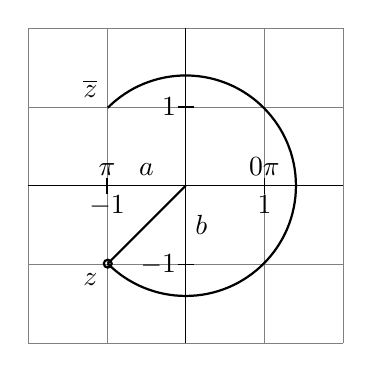
\begin{tikzpicture}
                  \coordinate (O) at (0,0);

                  % Ejes
                  \draw[very thin,gray] (-2,-2) grid (2,2);
                  \begin{scope}[thin]
                      \draw (-2,0) -- (2,0);
                      \draw (0,-2) -- (0,2);
                      \draw (1,0) node[anchor=north] {$1$};
                      \draw (-1,0) node[anchor=north] {$-1$};
                      \draw (0,1) node[anchor=east] {$1$};
                      \draw (0,-1) node[anchor=east] {$-1$};
                      \draw (1,-0.1) -- (1,0.1);
                      \draw (-1,-0.1) -- (-1,0.1);
                      \draw (-0.1,1) -- (0.1,1);
                      \draw (-0.1,-1) -- (0.1,-1);
                  \end{scope}

                  \begin{scope}[thick]
                      \draw (1,0) node [anchor=south] {$0\pi$};
                      \draw (-1,0) node [anchor=south] {$\pi$};
                      \draw (1.4,0) arc (0:135:1.4) node[anchor=south east] {$\overline{z}$};
                      \draw (1.4,0) arc (0:-135:1.4) node[anchor=north east] {$z$} circle[fill=black,radius=0.05] -- (O);
                  \end{scope}

                  \draw (0,-0.5) node[anchor=west] {$b$};
                  \draw (-0.5,0) node[anchor=south] {$a$};
              \end{tikzpicture}
          \end{center}
          \[
              \tan\left(\frac{5}{4}\pi\right) = a = -1
          \] \[
              z = -1 - i \implies \boxed{z^4 = -4}
          \]


    \item Determinar polinomio $P \in R[x]$ de grado mínimo que tiene una raíz doble, $i$ y $5$ son raíces de $P$ y $P(0) = -5$ \\
          Ya que el polinomio es real, pero tiene que tener una raiz imaginaria, uno de los terminos va a tener que ser $(x^2 + 1)$, que tiene $S = \{i, -i\}$. Aparte, para que tenga raiz en 5, va a tener un termino $(x-5)$, el cual podemos elevar al cuadrado para tener la raiz doble.
          \[ P(x) = a(x-5)^2(x^2+1) \]
          \[ P(0) = a(-5)^2(1) = 25a = -5 \implies a = -\frac{1}{5} \]
          \[ P(x) = -\frac{1}{5}(x-5)^2(x^2+1) \]

    \item Encontrar $a$ y $b$ para que el polinomio $P(x) = (2x-a)^2(bx-4)^3(x^2-3x+2)$ tenga a $1$ como raíz de multiplicidad $3$ % a=2 b!=4 / a!=2 b!=4 / a!=2 b=4 / a=2 b=4
          \[ (2x - a)^2 (bx - 4)^3 (x - 1)(x - 2) \]
          \[ P(1) = (2\cdot 1 - a)^2 (b\cdot 1 - 4)^3 (1 - 1)(1 - 2) = 0 \]
          \[ (2\cdot 1 - a)^2 = 0 = 2 - a \implies a = 2 \]
          \[ (b\cdot 1 - 4)^3 \neq 0 \implies b \neq 4 \]
          \[ \boxed{a = 2 \land a \neq 4} \]

    \item Sean $B = \{x, y, z, w\}$ una base de un espacio vectorial $V$ y $C = \{x + 2y + z,y + w,x + 3y + az + w,x + y + z + aw\}$. Encontrar el conjunto de todos los $a \in R$ tales que $C$ no es una base de $V$ % {-1} / {-1,1} / {-1,2} / R-{-1}
          \[
              C = \begin{pmatrix}
                  1 & 2 & 1 & 0 \\
                  0 & 1 & 0 & 1 \\
                  1 & 3 & a & 1 \\
                  1 & 1 & 1 & a
              \end{pmatrix}
              \equiv
              \begin{pmatrix}
                  1 & 0 & 1   & -2  \\
                  0 & 1 & 0   & 1   \\
                  0 & 0 & a-1 & 0   \\
                  0 & 0 & 0   & a+1
              \end{pmatrix}
          \]
          Si \(\text{rn} C < 4\) entonces \(C\) no es base de \(V\)
          \[ a - 1 = 0 \lor a + 1 = 0\]
          \[ a = 1 \lor a = - 1 \]
          \[ \boxed{S = \{-1, 1\}} \]

    \item Sean $\S = \{(x,y,z,w) \in \R^4 / x + y - z - 2z = 0; x - 2y + z = 0\}$ y $\T = \langle(1,1,1,0),(0,-1,2,-1)\rangle⟩$. Calcular $\S \cap \T$ % ⟨(1,0,3,-1)⟩ / ⟨(1,-1,-1,1)⟩ / {(0,0,0,0)} / ⟨(0,1,-3,2)⟩
          \[
              \T = a(1,1,1,0) + b(0,-1,2,-1) = (a, a-b, a+2b, -b)
          \] \[
              \begin{cases}
                  (a) + (a-b) - (a+2b) - 2(-b) = 0 \\
                  (a) - 2(a-b) + (-b) = 0
              \end{cases}
          \] \[
              \begin{cases}
                  a - b = 0 \\
                  -a + b = 0
              \end{cases}
              \implies
              a = b
          \] \[
              \S\cap\T = a(1,1,1,0) + a(0,-1,2,-1) = a((1,1,1,0) + (0,-1,2,-1)) = a(1,0,3,-1)
          \] \[
              \boxed{\S\cap\T = \langle(1,0,3,-1)\rangle}
          \]

    \item Sean $S = \{x \in R^4 / x + 2y - z = 0; -x + y + w = 0\}$ y $\T = \langle(1,-2,1,1),(2,1,0,3)\rangle$. Encontrar una base de $\S + \T$ % {(1,2,-1,0),(-1,1,0,1),(1,-2,1,1),(2,0,1,3)} / {(1,0,1,1),(0,1,2,-1),(1,-2,1,1)} / {(1,0,1,1),(0,1,2,-1),(1,-2,1,1),(2,1,0,3)} / {(1,2,-1,0),(-1,1,0,1),(1,-2,1,1)}
          \[
              \begin{cases}
                  x + 2y - z = 0 \\
                  -x + y + w = 0
              \end{cases}
              \equiv
              \begin{cases}
                  x + 2y = z \\
                  x - y  = w
              \end{cases}
          \] \[
              (x,y,z,w) = (x,y,x + 2y,x - y) = x(1,0,1,1) + y(0,1,2,-1)
          \] \[
              \S = \langle(1,0,1,1),(0,1,2,-1)\rangle
          \] \[
              \T+\S = \langle(1,-2,1,1),(2,1,0,3),(1,0,1,1),(0,1,2,-1)\rangle
          \] \[
              \begin{pmatrix}
                  1 & -2 & 1 & 1  \\
                  2 & 1  & 0 & 3  \\
                  1 & 0  & 1 & 1  \\
                  0 & 1  & 2 & -1 \\
              \end{pmatrix}
              \equiv
              \begin{pmatrix}
                  0 & -1 & 0 & 0  \\
                  0 & 0  & 0 & 0  \\
                  1 & 0  & 1 & 1  \\
                  0 & 0  & 2 & -1 \\
              \end{pmatrix}
          \]
          El 2º vector no es linealmente independiente, asi que lo eliminamos
          \[
              \T+\S = \langle(1,-2,1,1),(1,0,1,1),(0,1,2,-1)\rangle
          \]

    \item Sea $B = \{(1,2,1),(0,1,1),v\}$. Si $(-1,2,1)_B = (1,-1,1)$, entonces
          % v=(0,3,1) / v=(-1,-4,0) / v=(-2,1,1) / v=(2,-1,0)
          \[
              1(1,2,1) - 1(0,1,1) + 1v = (1,1,0) + v = (-1,2,1)
          \] \[
              v = (-1,2,1) - (1,1,0) = (-2,1,1)
          \] \[
              \boxed{v = (-2,1,1)}
          \]

    \item Sea $f : R^3 \to R^3$ la t. l. definida por $f(x) = (x + ky - z, -y + z, x + 3z)$. Calcular el valor de $k \in R$ para el cual $f(-5,1,2) \in \Nu(f)$
          % k=2 / k=4 / k=5 / k=3
          \[
              M(f) = \begin{pmatrix}
                  1 & k  & -1 \\
                  0 & -1 & 1  \\
                  1 & 0  & 3
              \end{pmatrix}
          \] \[
              f(-5,1,2) \in \Nu(f) \implies f\circ f(-5,1,2) = \0
          \] \[
              \begin{pmatrix}
                  1 & k  & -1 \\
                  0 & -1 & 1  \\
                  1 & 0  & 3
              \end{pmatrix}\cdot\begin{pmatrix}
                  1 & k  & -1 \\
                  0 & -1 & 1  \\
                  1 & 0  & 3
              \end{pmatrix}\cdot\begin{pmatrix}
                  -5 \\ 1 \\ 2
              \end{pmatrix} = \0
          \] \[
              (k-4)
              \begin{pmatrix}
                  2 \\ 0 \\ 1
              \end{pmatrix} = \begin{pmatrix}
                  0 \\ 0 \\ 0
              \end{pmatrix}
          \] \[
              \boxed{k = 4}
          \]

    \item Sean $B = \{(0,1,1),(0,1,-1),(1,0,0)\}$ base de $R^3$, $f : R^3 \to R^3$ la t. l. tal que $M_B(f)=\begin{pmatrix}
                  1 & 1 & 0 \\ 2 & -1 & 1 \\ 3 & 1 & -1
              \end{pmatrix}$ y $\S = \{x \in R^3 / x_2 = 0; x_3 = 0\}$. Calcular $f(\S)$
          % ⟨(0,1,-1)⟩ / ⟨(1,2,3)⟩ / ⟨(3,3,-1)⟩ / ⟨(-1,1,-1)⟩
          Primero escribimos $M(f)$ en el sistema de coordenadas estándar.
          \[
              M_{BB} = \begin{pmatrix}
                  0 & 0  & 1 \\
                  1 & 1  & 0 \\
                  1 & -1 & 0
              \end{pmatrix}
          \] \[
              M_{EE}(f) = C_{BE}\cdot M_{BB}(f) \cdot C_{EB}
          \] \[
              C_{BE} = \begin{pmatrix}
                  0 & 0  & 1 \\
                  1 & 1  & 0 \\
                  1 & -1 & 0 \\
              \end{pmatrix}
          \]
          \[
              C_{EB} = (C_{BE})^{-1} = \frac{1}{2}\begin{pmatrix}
                  0 & 1 & 1  \\
                  0 & 1 & -1 \\
                  2 & 0 & 0  \\
              \end{pmatrix}
          \] \[
              M_{EE}(f) = \begin{pmatrix}
                  0 & 0  & 1 \\
                  1 & 1  & 0 \\
                  1 & -1 & 0 \\
              \end{pmatrix}\cdot\begin{pmatrix}
                  1 & 1  & 0  \\
                  2 & -1 & 1  \\
                  3 & 1  & -1 \\
              \end{pmatrix}\cdot \frac{1}{2}\begin{pmatrix}
                  0 & 1 & 1  \\
                  0 & 1 & -1 \\
                  2 & 0 & 0  \\
              \end{pmatrix}
          \] \[
              M_{EE}(f)  =
              \frac{1}{2}
              \begin{pmatrix}
                  -2 & 4 & 2  \\
                  2  & 3 & 3  \\
                  -2 & 1 & -3 \\
              \end{pmatrix}
          \]
          Luego escribimos $\mathbb{S}$ como generador:
          \begin{align*}
              \mathbb{S} & =\begin{cases}
                  x_1=x_1 \\
                  x_2=0   \\
                  x_3=0
              \end{cases} \\
                         & =(x, 0, 0)                  \\
                         & =x(1, 0, 0)                 \\
                         & =\langle(1, 0, 0)\rangle
          \end{align*}
          Y aplicamos la transformación:
          \begin{align*}
              f(\mathbb{S}) & =M(f)\cdot\mathbb{S}                                                                               \\
                            & =\frac{1}{2}\begin{pmatrix}
                  -2 & 4 & 2  \\
                  2  & 3 & 3  \\
                  -2 & 1 & -3 \\
              \end{pmatrix}\cdot\begin{pmatrix}
                  1 \\
                  0 \\
                  0
              \end{pmatrix} = \begin{pmatrix}
                  -1 \\
                  1  \\
                  -1
              \end{pmatrix}
          \end{align*}
          \[ \boxed{f(\S) = \langle(-1,1,-1)\rangle} \]


    \item Sea $B = \{(1,1,1),(-3,1,2),(-1,0,0)\}$ base de $R^3$ y sea $f : R^3 \to R^3$ la t. l. tal que $M_{BE} = \begin{pmatrix}
                  -1 & 2 & 3 \\ 1 & 0 & 1 \\ 0 & 1 & 2
              \end{pmatrix}$.
          Calcular $\Nu f$ \\
          % Nu(f)={(0,0,0)} / Nu(f)=⟨(1,2,-1)⟩ / Nu(f)=⟨(-4,3,5)⟩ / Nu(f)=⟨(5,-3,13)⟩
          Primero hay que convertir $M_{BE}$ a $B_{EE}$
          \[ M_{EE} = M_{BE}(f) \cdot C_{EB} \]
          \[
              C_{EB} = (C_{BE})^{-1} = \begin{pmatrix}
                  1 & -3 & -1 \\
                  1 & 1  & 0  \\
                  1 & 2  & 0  \\
              \end{pmatrix}^{-1} = \begin{pmatrix}
                  0  & 2  & -1 \\
                  0  & -1 & 1  \\
                  -1 & 5  & -4 \\
              \end{pmatrix}
          \] \[
              M_{EE} = M_{BE}(f) \cdot C_{EB}
          \] \[
              M_{EE} = \begin{pmatrix}
                  -1 & 2 & 3 \\
                  1  & 0 & 1 \\
                  0  & 1 & 2 \\
              \end{pmatrix}\cdot\begin{pmatrix}
                  0  & 2  & -1 \\
                  0  & -1 & 1  \\
                  -1 & 5  & -4 \\
              \end{pmatrix} = \begin{pmatrix}
                  -3 & 11 & -9 \\
                  -1 & 7  & -5 \\
                  -2 & 9  & -7 \\
              \end{pmatrix}
          \] \[
              \text{Diagonalizada: }
              \begin{pmatrix}
                  -1 & 2 & -2 \\
                  0  & 5 & -3 \\
                  0  & 0 & 0  \\
              \end{pmatrix}
          \] \[
              \begin{pmatrix}
                  -1 & 2 & -2 \\
                  0  & 5 & -3 \\
                  0  & 0 & 0  \\
              \end{pmatrix} = \begin{pmatrix}
                  0 \\ 0 \\
              \end{pmatrix}
          \] \[
              \begin{cases}
                  -x + 2y - 2z = 0 \\
                  5y - 3z = 0      \\
              \end{cases}
              \implies
              \begin{cases}
                  2y - 2z = x      \\
                  \frac{3}{5}z = y \\
              \end{cases}
          \] \[
              (x,y,z) = \left(\frac{6}{5}z - 2z, \frac{3}{5}z, z\right) = z\left(\frac{-4}{5}, \frac{3}{5}, 1\right) \equiv z(-4,3,5)
          \] \[
              \boxed{\Nu f = (-4,3,5)}
          \]

    \item Sea $B = \{x,y,z\}$ una base de un espacio vectorial $V$ y sea $f : V \to V$ la t. l. tal que $M_B(f) = \begin{pmatrix}
                  0 & 0 & 0 \\ 0 & 0 & 1 \\ 1 & 0 & 0
              \end{pmatrix}$. La imagen de $f \circ f$ es
          % ⟨y⟩ / ⟨y,z⟩ / ⟨x⟩ / ⟨x,z⟩
          \[ M_{EE}(f) = C_{BE}\cdot M_{BB}(f)\cdot C_{EB} \]
          \[
              f \circ f = \begin{pmatrix}
                  0 & 0 & 0 \\ 0 & 0 & 1 \\ 1 & 0 & 0
              \end{pmatrix}\cdot\begin{pmatrix}
                  0 & 0 & 0 \\ 0 & 0 & 1 \\ 1 & 0 & 0
              \end{pmatrix} = \begin{pmatrix}
                  0 & 0 & 0 \\
                  1 & 0 & 0 \\
                  0 & 0 & 0
              \end{pmatrix}
          \]
          Asumimos que las bases de $B$ son en realidad las bases canonicas
          \[
              f \circ f(x) = \begin{pmatrix}
                  0 & 0 & 0 \\
                  1 & 0 & 0 \\
                  0 & 0 & 0
              \end{pmatrix}\begin{pmatrix}
                  1 \\ 0 \\ 0
              \end{pmatrix} = \begin{pmatrix}
                  0 \\ 1 \\ 0
              \end{pmatrix}
          \] \[
              f \circ f(y) = \begin{pmatrix}
                  0 & 0 & 0 \\
                  1 & 0 & 0 \\
                  0 & 0 & 0
              \end{pmatrix}\begin{pmatrix}
                  0 \\ 1 \\ 0
              \end{pmatrix} = \begin{pmatrix}
                  0 \\ 0 \\ 0
              \end{pmatrix}
          \] \[
              f \circ f(z) = \begin{pmatrix}
                  0 & 0 & 0 \\
                  1 & 0 & 0 \\
                  0 & 0 & 0
              \end{pmatrix}\begin{pmatrix}
                  0 \\ 0 \\ 1
              \end{pmatrix} = \begin{pmatrix}
                  0 \\ 0 \\ 0
              \end{pmatrix}
          \] \[
              \boxed{\Img f \circ f = \langle y \rangle}
          \]

    \item Sea $A = \begin{pmatrix}
                  3 & a & 0 \\ b & 2 & -3 \\ 2 & 0 & 1
              \end{pmatrix}$. Encontrar los valores de $a$ y $b$ para los cuales $(1,-1,1)$ es un autovector de $A$
          % a=2, b=4 / a=2, b=6 / a=0, b=8 / a=0, b=2
          \[
              Av = \lambda v
          \] \[
              \begin{pmatrix}
                  3 & a & 0 \\ b & 2 & -3 \\ 2 & 0 & 1
              \end{pmatrix}
              \begin{pmatrix}
                  1 \\ -1 \\ 1
              \end{pmatrix}
              =
              \lambda
              \begin{pmatrix}
                  1 \\ -1 \\ 1
              \end{pmatrix}
          \] \[
              \begin{pmatrix}
                  3 - a \\ b - 5 \\ 3
              \end{pmatrix}
              =
              \begin{pmatrix}
                  \lambda \\ -\lambda \\ \lambda
              \end{pmatrix}
          \] \[
              \begin{cases}
                  3 - a = \lambda  \\
                  b - 5 = -\lambda \\
                  3 = \lambda
              \end{cases}
          \] \[
              \begin{cases}
                  3 - a  = 3 \\
                  b - 5 = - 3
              \end{cases}
              \implies
              \begin{cases}
                  a = 0 \\
                  b = 2
              \end{cases}
          \] \[
              \boxed{a = 0 \land b = 2}
          \]

    \item Sea $A = \begin{pmatrix}
                  -2 & 0 & 0 \\ 1 & 5 & 3 \\ 0 & -6 & -4
              \end{pmatrix}$. Existe una matriz inversible $C \in R^{3\x3}$ tal que $A = CDC^{-1}$ si: \\
          \begin{enumerate*}
              \item $ D = \begin{pmatrix}
                      -1 & 0 & 0  \\
                      0  & 2 & 0  \\
                      0  & 0 & -2
                  \end{pmatrix} $
              \item $ D = \begin{pmatrix}
                      -1 & 0 & 0 \\
                      0  & 2 & 0 \\
                      0  & 0 & 2
                  \end{pmatrix} $
              \item $ D = \begin{pmatrix}
                      1 & 0  & 0 \\
                      0 & -2 & 0 \\
                      0 & 0  & 2
                  \end{pmatrix} $
              \item $ D = \begin{pmatrix}
                      1 & 0  & 0  \\
                      0 & -2 & 0  \\
                      0 & 0  & -2
                  \end{pmatrix} $
          \end{enumerate*} \\
          Encontrar autovectores de $A$:
          \begin{align*}
              v_1 & = (-2, -1, 3) \\
              v_2 & = (0, -1, 1)  \\
              v_3 & = (0, -1, 2)  \\
          \end{align*}
          Verificar que sean l. i.:
          \[
              \begin{pmatrix}
                  -2 & -1 & 3 \\
                  0  & -1 & 1 \\
                  0  & -1 & 2 \\
              \end{pmatrix}
              \implies
              \begin{pmatrix}
                  -2 & 0  & 0 \\
                  0  & -1 & 0 \\
                  0  & 0  & 1 \\
              \end{pmatrix}
          \] \[
              \boxed{D = \begin{pmatrix}
                      -2 & 0  & 0 \\
                      0  & -1 & 0 \\
                      0  & 0  & 1 \\
                  \end{pmatrix}}
          \]

\end{enumerate}

\end{document}